Aside from the standard connected to the visualization of raster data there are also standard for the formatting of the raster files. Common raster formats include jpeg, png and tiff. One of the key differences between these formats are the bit depth. This value determines how many different colors that can be assigned each pixel in the image. Each bit can only be assigned one of two values, 0 or 1. This number of available colors for a pixel can therefore be calculated as $2^{number of bits}$. As an example, a bit depth of 8 bits would then result in $2^8 = 256$ different potential colors, since is the number of combinations of ones and zeroes, that are possible. For most maps this amount of colors is enough. The human eye can comprehend around 10 million different colors, but often that many colors are not needed. When displaying aerial photographs, the depth of 24 bits is often used, since it can display 16.7 million different colors and therefore can appear in true-colors to humans.
The limitations of the human eye does not mean that having more than 10 million bit combination is pointless. The bit combination can also be used for other thing than colors. It can be used to create transparency values or to store metadata about the image file. For instance, the geotiff format can use the additional bit to store georeferencing information.
These advantages of higher bit count come at a cost of a larger file size. Having a larger color depth will result in a slower loading and larger requirements for storage space.
Dent. 283 
\section{Tiled raster}
This section describes standards for dividing large raster files into smaller tiles. 
A way of only visualising the necessary parts of a raster is to divide it into smaller raster tiles and then only load the relevant tiles. When loaded into the map these tiles then gets places next to eachother, so they appear as a single large map image. These tiles can also be created with different resolutions, so that zooming in on the map with return tiles more details.  As illustrated in figure \ref{TilesPerZoomLevel} each of these zoom layers have more tiles.
 http://www.liedman.net/tiled-maps/
When zoomed all the way out the entire world is rendered as a single tile. Whenever the zoom level gets increased by one each tile in the previous layer get replaced with four smaller tiles. The number of tiles on a zoom level z can therefore be calculated as $2^2z$

$https://wiki.openstreetmap.org/wiki/Slippy_map_tilenames$
 

\begin{figure} [H]
	\centering
	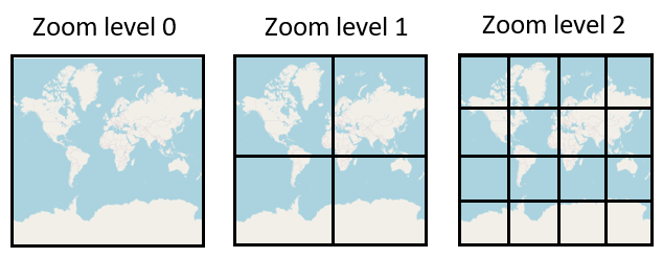
\includegraphics[width=.8\textwidth]{Pictures/TilesPerZoomLevel}
	\caption{Illustration of the increase in tiles for each zoom level}
	\label{TilesPerZoomLevel}
\end{figure}

Openstreetmaps is an example of a service, which use tiled rasters for their map. When this service is used, requests for tiles are send to 
http://tile.openstreetmap.org/zoom/x/y.png
In the request the values zoom, x and y are replaced with the current zoom level, tile column and tile row.
$https://wiki.openstreetmap.org/wiki/Slippy_map_tilenames$
 
 \begin{figure} [H]
 	\centering
 	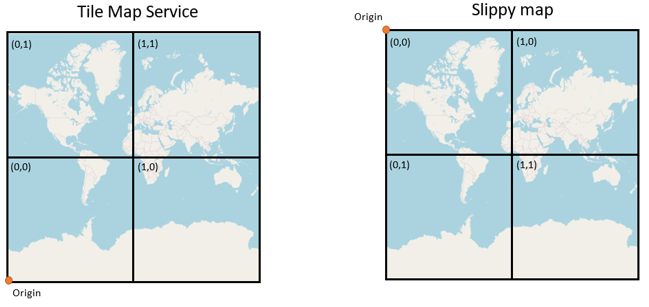
\includegraphics[width=.8\textwidth]{Pictures/TMSXYZ}
 	\caption{Illustration of the difference between the TMS and XYZ formats}
 	\label{TMSXYZ}
 \end{figure}
 
 %https://developers.planet.com/tutorials/slippy-maps-101/ https://wiki.osgeo.org/wiki/Tile_Map_Service_Specification#TileMap_Diagram 

The naming of these tiles are done differently for different standards. In this section only the Tile Map Service (TMS) and Slippy map (XYZ) standard will be addressed. Both of these have the same approach to naming zoom level and columns, but different approach to naming the rows. This difference has been illustrated in figure \ref{TMSXYZ}. The reason for the difference is that TMS tiles number their rows from south northwards, whereas XYZ are numbering rows the reverse way. Due to this difference in numbering rows loading tiles from the wrong standard results in a map as shown in figure \ref{SlippyInTMS}.
https://wiki.openstreetmap.org/wiki/TMS 
 
 
 \begin{figure} [H]
 	\centering
 	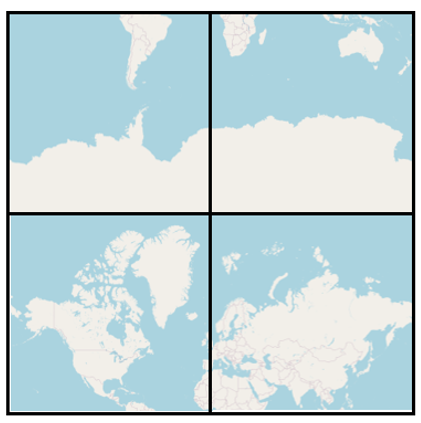
\includegraphics[width=.8\textwidth]{Pictures/SlippyInTMS}
 	\caption{How the map looks, when the TSM and XYZ get switched}
 	\label{SlippyInTMS}
 \end{figure}
 
\chapter{Initial research and related work}

Prior to developing the tool some initial experimentation with the case dataset was conducted. This lead to some core concepts which should apply to the developed tool. After this existing tool is described, which follows many of these core concepts.

\section{Core concepts}

Based on the initial research and tests a four core concepts were developed:
\begin{itemize}
 \item Load only the needed data
 \item Coloring should be based on the current extent
 \item Tiles should not be precolored
 \item Coloring should be done locally
 \item File format should have same bit depth as input format
\end{itemize}


\section{Load only the needed data}
The case data presented in chapter x holds information for the entire world. However, loading data for the entire world would be unnecessarily time consuming. Initial experiments of rendering this quantity of data also revealed that the browser did not have enough memory to load that amount of data. Instead only the relevant data should be downloaded. The relevant data in this case would refer to the data, which the user is able to see. Getting a subset of a raster dataset can be accomplished by dividing it into smaller tiles. Section x will present two different ways this can be achieved. 

\section{Coloring should be based on the current extent}
The initial exploration of the data showed that the coloring of the tiles should be based of the current extent. This is due to the how much the values are varying across the world. Figure \ref{WhyLimitToExtent} shows an example of the difference between a map where the coloring is based on all values or if it is limited to the current extent. Both maps illustrate the population in Denmark. The left map has its coloring based on values from the entire world, while the right has its colors based on the current extent. The left map appears empty since the population density in Denmark is negligible compared with the densest areas in the world. In the right map it is possible to see the location of the most populated cities. Since the left map provide the user with no relevant information and the right one does, the coloring should be based on the current extent.
 
 
\begin{figure} [H]
	\centering
	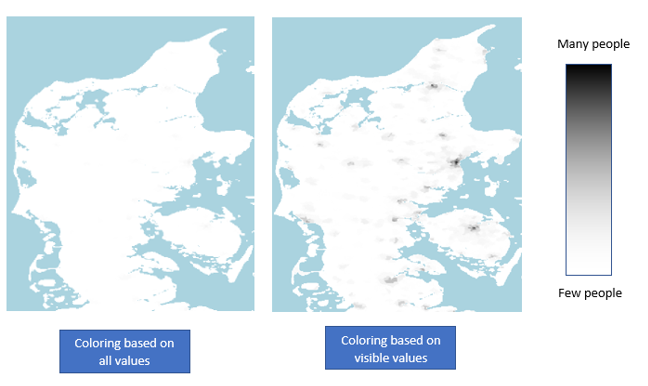
\includegraphics[width=.8\textwidth]{Pictures/WhyLimitToExtent}
	\caption{Population density in Jutland}
	\label{WhyLimitToExtent}
\end{figure}




\section{Tiles should not be precolored}
If the coloring should be based on the current extent and the map is interactive the coloring of the tiles should be done on the fly instead of once and for all. The reason for this is best explained with the example in figure \ref{WhyNotPrecolor}. This figure is illustrating the population in a small subset of India.  The three boxes are illustrating examples of possible map extents, which the user could get by zooming in on different parts of the map. Each of these three have a different max value in their cell with the highest population. The blue square is covering the city center of Indore a therefore have a high value than the green, which is covering the outskirts of the city. The last square does not include any part of a bigger city and therefore have a lower value. 
Since their max values are different, they would each need their own coloring. If the tiles were to be precolored it would be necessary, create three coloring of the tiles – one for each the extents. However, since the map is interactive, the extent is not limited to those three. If the user instead were to zoom in on an area between the red and blue square a new max value would maybe be found. When scaling this example up to the entire world and to multiple zoom extents there would be thousands of combinations. If all of these needed to be prerender it would both require lots of initial processing time and storage space for an immense amount of data. 
 
 
\begin{figure} [H]
	\centering
	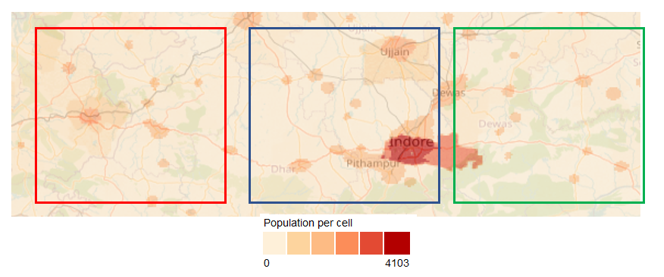
\includegraphics[width=.8\textwidth]{Pictures/WhyNotPrecolor}
	\caption{Population density. The three boxes are examples of possible extents an interacting user could get by zooming.}
	\label{WhyNotPrecolor}
\end{figure}

The alternative is to color the tiles on the fly. When the user would zoom to a new area the map, a script could register the highest currently visible value. This information could then be sent to recoloring script, which would color the tiles based on this. This way only tiles with the needed colors would be rendered. 


\section{Coloring should be done locally}
The coloring can be done in two ways as illustrated in figure \ref{WhyColorLocally}. It can be done by sending the information to a tileserver, which then would color the tiles and send them to the client. Alternatively, the coloring could be done on the client. 
 
 \begin{figure} [H]
 	\centering
 	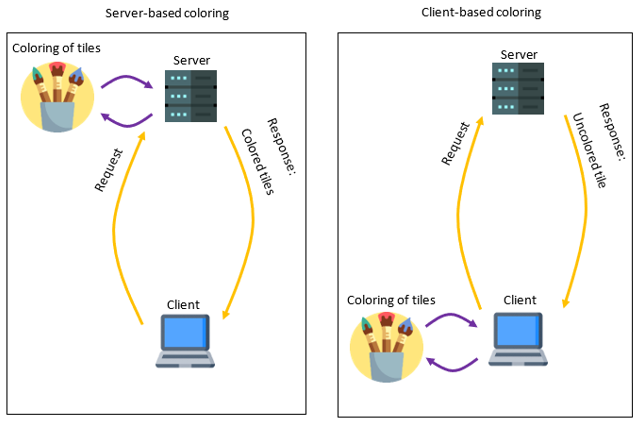
\includegraphics[width=.8\textwidth]{Pictures/WhyColorLocally}
 	\caption{Difference between coloring the tile on the server and locally}
 	\label{WhyColorLocally}
 \end{figure}
 
Comparing the two options is best done with an example, which has been illustrated in figure \ref{WhyColorLocallyMap}. Here the blue and green box are two different possible views both containing 16 raster tiles. The two boxes have different max values, since blue one contains the city center. In the example a user will pan from the blue view to the green one. If the coloring is done on the server side the initial 16 tiles in the blue box will be requested on load. Then when the user pan to the green view the 16 tiles in that box will be requested and colored. The four tiles that are shared between the blue and the green boxes must be requested again, since they need a new color due to the change in max value. This is not the case if the coloring is done locally. In this case only 12 tiles would have to be requested, when changing from the blue to the green view. Since the coloring is happening locally the coloring script can recolor the four tiles it already has downloaded from the initial load. This should result in a faster experience for the user.
   
\begin{figure} [H]
	\centering
	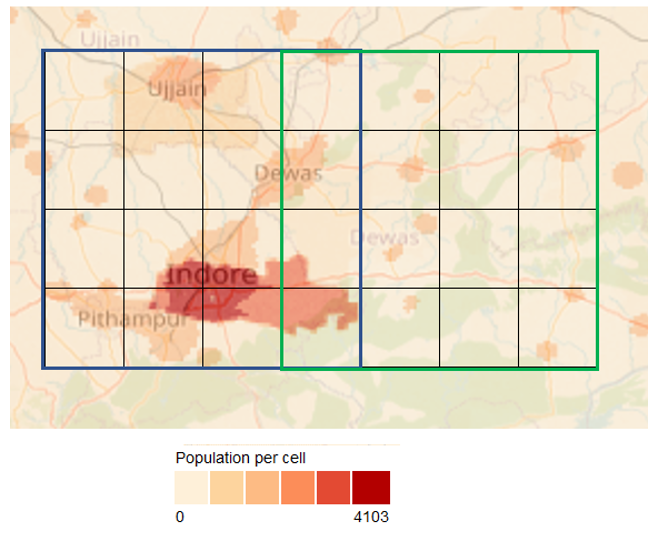
\includegraphics[width=.8\textwidth]{Pictures/WhyColorLocallyMap}
	\caption{Example of why local coloring is needed. The squares are different extents used for the example}
	\label{WhyColorLocallyMap}
\end{figure}

\section{File format should have same bit depth as input format}
As mention in section x the data from the case has a bit depth of 32 bit. To visualize the data the file format must not be changed to a format with less than 32 bits. Figure \ref{WhyColorLocallyMap} is an example of how a subset of the case data look originally and when converted to an 8-bit format. As mentioned in section x the pixels in an 8-bit raster can have values between 0-255. This means that this format is unable to correctly display the original data range, where the data range is covering thousands of values. The original data get clamped into the 8-bit format producing wrong result
https://gdal.org/programs/gdal2tiles.html .
 
 \begin{figure} [H]
 	\centering
 	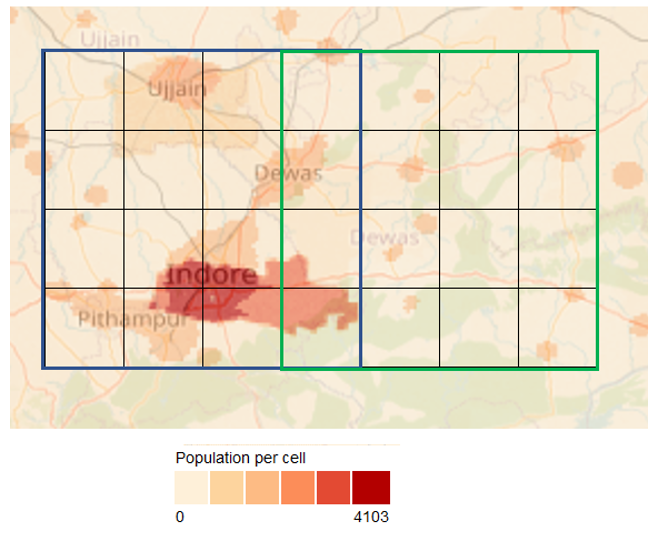
\includegraphics[width=.8\textwidth]{Pictures/WhyColorLocallyMap}
 	\caption{32 bits cramped into 8 bits}
 	\label{WhyColorLocallyMap}
 \end{figure}
 
Normally this issue could be worked around by rescaling the input data to the new format https://gdal.org/programs/gdal2tiles.html . This rescaling would be a lossy compression resulting in loss of information since the original data cannot be expressed with values between 0-255. \citep{dent}
For the normal use of tiles this would not be a problem since tiles would only be used for visualization. 
If the tiles are being recolored locally the tiles are being used for more than just visualization. It is necessary to access the data within the tile. This means that solutions resulting in a lossy compression are not an option. To ensure that the correct data reach the client the file format used for tiles must have a bit depth of 32. 
  






\section{Related work}
This is not the first project to follow many of these core concepts. In Bernhard Baumrocks master thesis, he created a webmap, where raster tiles were being colored locally. \citep{Buamrocks}
\begin{figure} [H]
	\centering
	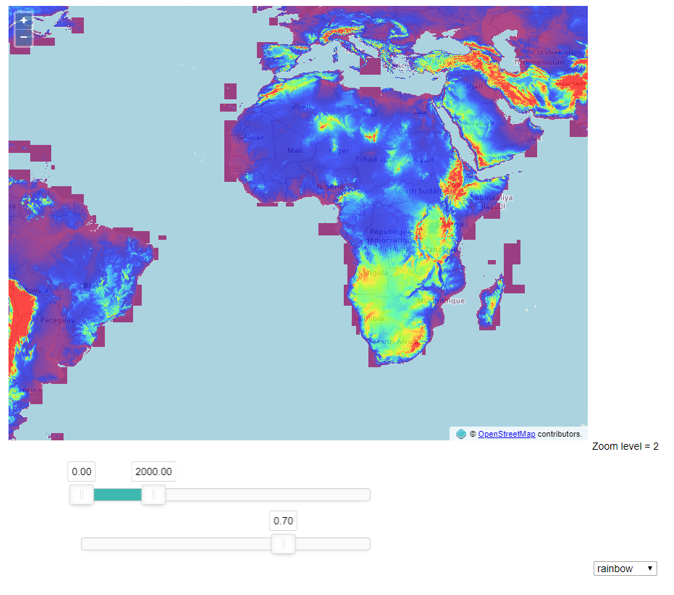
\includegraphics[width=.8\textwidth]{Pictures/BaumrockMap1}
	\caption{The map created by Bernhard Baumrock}
	\label{BaumrockMap1}
\end{figure}

A picture of one of his maps can be seen in figure \ref{BaumrockMap1}. This particular map is not included in his thesis, but it is the most similar to this project. The map shows an unspecified dataset colored in rainbow colors. Below the map are two sliders and a dropdown list with the label “rainbow”. Changing the value in this dropdown list allows the user to switch to another color scheme. The bottom slider is controlling the opacity for the raster layer. The upper slider controls which maximum and minimum values the coloring should be based on. How the map change, when changing the values in the upper slider can be seen in figure \ref{BaumrockMap2}. When zooming in another more detailed layer gets loaded and rendered.
\begin{figure} [H]
	\centering
	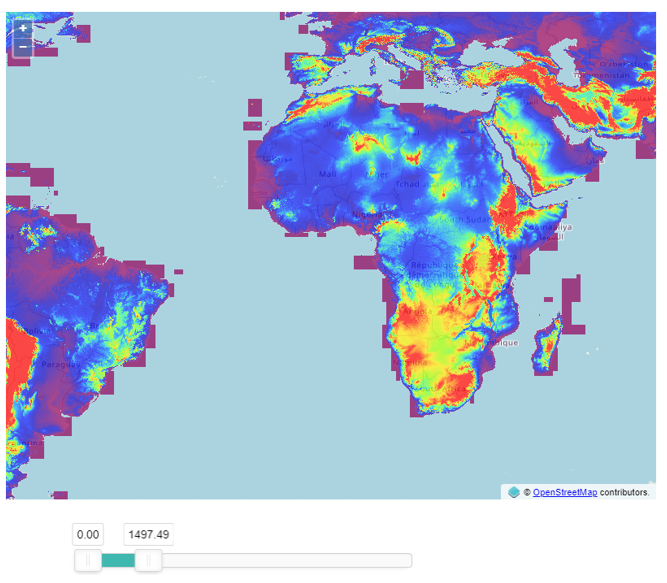
\includegraphics[width=.8\textwidth]{Pictures/BaumrockMap2}
	\caption{How the map change, when using the slider}
	\label{BaumrockMap2}
\end{figure}


%http://webportals.ipsl.jussieu.fr/ScientificApps/dev/forge_patrick/eox/map_01.html
 
When taking a closer look at the source code it can be seen that the raster is being loaded as tiff tiles with a bit depth of 16 bit. \citep{BuamrocksSouce} Only tiles the currently are visible are being requested unless the tile already have been requested. \citep{Buamrocks}

When comparing with the core concepts for this project, Baumrocks map fulfil most of the criteria. It is locally visualizing only the necessary data. The core concept related to bit depth is relevant in the creation of the tiles, so it does not really apply to this. 
It is also to some extent allowing the user to color the layer based on the current extent. The user can adjust the maximum and minimum values but does not know what the maximum values are in the current extent. 
How the tool functions from a technical perspective is further detailed in section x.

\section{Sections to be written here} 

Other ways of trying to visualizing large rasters:

\begin{itemize}
	\item qgis
	\item makeCitywebsite?
	\item Visualing with bokeh or folium 
\end{itemize}

Benchmarking using google lighthouse


\part{Development of the tool}
In this chapter it is explained how the tool has been developed. The first section is describing the coding languages used and the plugins used to create the tool. The following sections are describing the necessary steps to build the tool. These steps can be seen in figure \ref{DevelopmentSteps}.
 
 \begin{figure} [H]
 	\centering
 	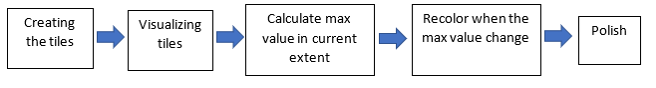
\includegraphics[width=.8\textwidth]{Pictures/DevelopmentSteps}
 	\caption{An overview of the code}
 	\label{DevelopmentSteps}
 \end{figure}
 
First it is necessary to divide the raster into tiles to be able to limit the loaded data to the current extent. How this is done is explained in section x. Section x describes how the tiles have been visualized. To be able to color the tiles based on the current values it is required to know what the current values are. In section x it is explained how this information is calculated. The raster layer is then rerendered with these values as described in section x. Lastly some measurements were taken to ensure a more user-friendly experience. These additions are described in section x. 

\chapter{Coding languages and plugins}
For this project, the coding language Python was used to create the tiles, while visualization of the tiles was done in a webgis build with the languages HTML, CSS and Javascript. This webgis have been tested on a local caddy server for reasons explained in section x

\section{Languages}
\subsection*{Python}
Python is programming language with a simple syntax, which functions across multiple different platforms. This simple syntax means that Python can achieve the same as some other coding languages in fewer lines. $https://www.w3schools.com/python/python_intro.asp$
Python was used in this project because of the gdal library expanded further upon in section x
This project has been using version 3.6 of Python. 
\subsection*{HTML}
HTML is short for Hyper Text Markup Language. It is the language used for defining and structuring a web page’s content.
https://www.w3schools.com/js/default.asp
\subsection*{CSS}
CSS is an abbreviation for Cascading Style Sheets. This language defines how the HTML will be displayed.
\subsection*{Javascript}
How a webpage behaves is defined by the language Javascript.  This is what makes the web page interactive. 
\citep{CPL}

\section{Libraries}
To transform the raster data into smaller tiles the python library Gdal is used. 
\subsection*{Gdal}
GDAL is library for translating between multiple different geospatial data formats. https://gdal.org/ 

Included in this library is the gdal2tiles program, which can divide raster files into smaller tiles. 
At the time of using this program it was only able to generate tiles structured after the TMS standard. The function to follow the XYZ structure was added the 3th of May 2020 https://gdal.org/programs/gdal2tiles.html
%https://gdal.org/download.html#current-releases 
The script rendering the tiles in the map was based on the XYZ structure. This meant that the rows of tiles were ordered incorrectly when the generated tiles were imported. Therefore, the official version of gdal2tiles was replaced by a version made by a github user named commenthol. This version is modified to allow the creation of tiles following the XYZ structure. 
https://github.com/commenthol/gdal2tiles-leaflet
Both the official version and the modified version have their output format as mbtiles with a bit depth of 8 bit. To be usable for this project a bit depth of at least 32 bit is needed, as mentioned in section x. The workaround for this issue will be explained in section x. 
\subsection*{Openlayers}
The map in which the tiles are being showed are created in Openlayers, which is an open source JavaScript library for creating dynamic maps for web pages. 
https://openlayers.org/
Openlayers was chosen because the tool presented in related work was built in Openlayers. Therefore, using Openlayers would enable expanding upon this existing tool instead of starting from scratch. 

\subsection*{olGeoTiff}
olGeoTiff is a Javascript class for visualising geotiff tiles in Openlayers, utilising the libraries geotiff.js and Plotty. The visualized tiles are being processing in the client instead of on a server. It was used in the map presented in section x. 
The class is a modified version of Openlayers WMTS layer, where the internal tile loading function has been changed. The regular function would request precolored tiles and then add them to the map. The tiles requested by the modified version are not precolored and need to be processed before getting added to the map. A simplified illustration of this processing is illustrated in figure x. This simplified figure is enough to explain the mechanics of the class but does not detail the callback function structure. Aside from being used for error handling callbacks are also necessary to ensure that Openlayers do not try to add the tiles to the map, before they have been processed. More detailed figures can be found in Bernhard Baumrocks thesis.
 
 \begin{figure} [H]
 	\centering
 	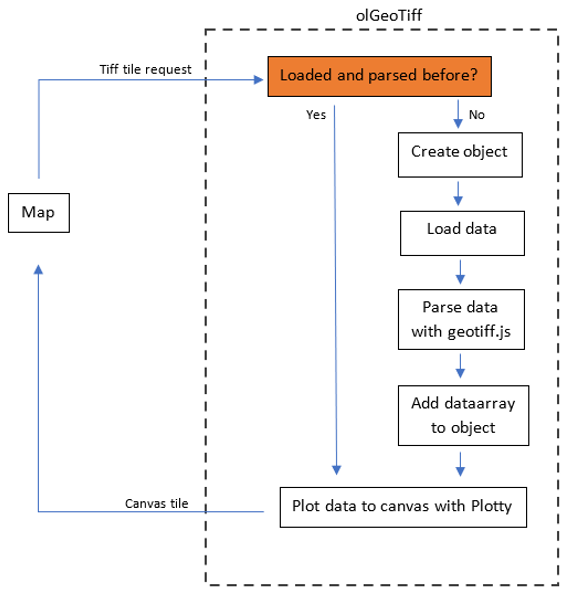
\includegraphics[width=.8\textwidth]{Pictures/olGeoTiffSimplified}
 	\caption{A simplified illustration of how olGEoTiff functions}
 	\label{olGeoTiffSimplified}
 \end{figure}
 
To ensure that tiles are only being downloaded once an object keeps track of all the downloaded data. The object is organized by the tiles’ url. 
Whenever tiles are being requested the object will always be checked to see if it already contains the url. If it does not the object will be updated to include the requested tile. The tile will then be loaded before being processed. 
The processing is done with the TIFF parser geotiff.js 
https://geotiffjs.github.io/
and Plotty, which is a library for creating images from data arrays.
https://github.com/santilland/plotty
. The loaded tiles first get parsed with geotiff.js and added to the object before Plotty get used to render tiles in the designated colors. Then the tiles get added to the map.
\citep{BThesis}
https://web.archive.org/web/20191031034339/https://eox.at/2018/01/visualizing-geotiff-tiles-with-openlayers/
The olGeoTiff also have a redraw function, which when triggered will redraw the tile layer based on the current designated colors. This was for instance used in Bernnard Baumrocks map, whenever the color sliders were changed. 

%\section{Testserver}
%Not finished
%The solution was being tested in Google Chrome initially using a python-based http server. This was later replaced with a Caddy server to improve performance. 
% 
%Caddy
%http’s limits to 6 connections 
%fig text: Blue: DomContentLoaded Red: Load

\chapter{Developing the tool}
This chapter details how the visualization tool was built.

\section{Creating the tiles}
The tiles got created using a modified version of gdal2tiles, which was changed to create tiles following the XYZ format. However, since the default output bit depth is too low, it would have to be modified further. The file format would also have to be changed to tiff in order to be visualized with the geotiff.js library. 

\subsection{Changing the file type}
Changing the file format can be done by changing two lines in the gdal2tiles script:

\begin{lstlisting}[language=iPython, caption={Changing the file format}, label= VoresPY,escapechar=|]
 #Original code
#self.tiledriver = 'PNG'
#self.tileext = 'png'
#New code
self.tiledriver = 'GTiff'
self.tileext = 'tiff'
\end{lstlisting}
This changes the raster driver from png to the geotiff format and the file extension from png to tiff. 
https://gdal.org/drivers/raster/index.html
The geospatial information, which is the difference between a geotiff and a regular tiff, gets lost in process. This information is not important for this project since the tiles are being loaded based on their name and folder placement, not based on the internal metadata.

Running gdal2tiles with these changes will produce a tiff file, which still would be limited to 8 bits. 
\subsection{Increasing the bit depth}
The reason for the bit limit is that gdal2tiles uses the memory dataset driver, which have 8 bits as default.  This default can overwritten to 32 bits by adding “gdal.GDT\_Int32” to every instance where the driver is being used as demonstrated in code x. 
http://osgeo-org.1560.x6.nabble.com/gdal-dev-gdal2tiles-for-16bit-data-tp5163094p5163098.html

\begin{lstlisting}[language=iPython, caption={Increasing the bit depth}, label= VoresPY,escapechar=|]
self.mem_drv = gdal.GetDriverByName('MEM')
...
#Old code
#dstile = mem_drv.Create('', tile_size, tile_size, tilebands)
#New code
dstile = self.mem_drv.Create('', self.tilesize, self.tilesize, tilebands, gdal.GDT_Int32)
\end{lstlisting}
The memory driver is being used four times, which all have been changed in a similar fashion.

Running the script with these changes produces tiles with the correct format and bit depth. The script also produces an xml file with metadata. An example of the content of said metadata file can be seen in code x.

\begin{lstlisting}[language=HTML5, caption={The metadata from the xml file generated by the modified gdal2tiles}, label= VoresHTML,escapechar=|]
<?xml version="1.0" encoding="UTF-8"?>
<TileMap tilemapservice="http://tms.osgeo.org/1.0.0" version="1.0.0"><Abstract/><SRS>GEOGCS["WGS 84",DATUM["WGS_1984",SPHEROID["WGS 84",6378137,298.257223563,AUTHORITY["EPSG","7030"]],
AUTHORITY["EPSG","6326"]],PRIMEM["Greenwich",0,AUTHORITY["EPSG","8901"]],UNIT["degree",0.0174532925199433,
AUTHORITY["EPSG","9122"]],AXIS["Latitude",NORTH],AXIS["Longitude",EAST],AUTHORITY["EPSG","4326"]]
</SRS><BoundingBox maxy="25.00000000000814" maxx="80.99999999999989" miny="19.00000000000815" minx="72.99999999999989"/><Origin y="19.00000000000815" x="72.99999999999989"/><TileFormat extension="tiff" mime-type="image/tiff" height="256" width="256"/><TileSets profile="raster"><TileSet order="2" units-per-pixel="0.00833333333333" href="2"/><TileSet order="3" units-per-pixel="0.00416666666667" href="3"/><TileSet order="4" units-per-pixel="0.00208333333333" href="4"/><TileSet order="5" units-per-pixel="0.00104166666667" href="5"/><TileSet order="6" units-per-pixel="0.00052083333333" href="6"/><TileSet order="7" units-per-pixel="0.00026041666667" href="7"/><TileSet order="8" units-per-pixel="0.00013020833333" href="8"/><TileSet order="9" units-per-pixel="0.00006510416667" href="9"/></TileSets></TileMap>
\end{lstlisting}


How long time did it take to run?

Running it parallelly it parallelly 

\section{Visualizing tiles}
After the tiles got created, they are stored in a folder, which gets uploaded to the testserver along the index file. 
The metadata from the xml file must be loaded into the map to be able to visualize the tiles. Normally this could be done using the WMTSCapabilities() function in Openlayers.
https://openlayers.org/en/latest/examples/wmts-layer-from-capabilities.html 
However, the formatting of the xml file produced by gdal is different from the format, which this function can read. Therefore, a small script has been created to parse the xml file and store the information in a metadata object. This object, tileMetadata, stores the bounding box, origin, center coordinates as well as tilesize. The initial version of the object also stored the resolution data, which is called units-per-pixel in code x. This led to some inconsistency when loading tiles, which had been generated without some of the lower zoom level. This will be further expanded upon in section x. Therefore, the resolution was instead generated using the script x, where 0.0333 is the value for units-per-pixel at zoom level 0. 

\begin{lstlisting}[language=JavaScript, caption={The JavaScript in the project}, label= VoresJS,escapechar=|]
for (var z = 0; z < 14; ++z) {
  // generate resolutions and matrixIds arrays for this WMTS
  //The number in the resolution calculation is the units-per-pixel value at zoomlayer 0 in the xml file generated by gdal2tiles
  resolutions[z] = 0.03333333333514 / Math.pow(2, z);
  matrixIds[z] = z;
}
\end{lstlisting}
Using this metadata, the tiles could be visualized using the olGeoTiff class. 

%\begin{lstlisting}[language=JavaScript, caption={The JavaScript in the project}, label= VoresJS,escapechar=|]
%var wmslayer = new ol.layer.Tile({
%  source: new ol.source.WMTS({
%    url: tileFolders + '/{TileMatrix}/{TileCol}/{TileRow}.tiff',
%    projection: projection,
%    tileGrid: new ol.tilegrid.WMTS({
%      origin: tileMetadata[origin],
%      resolutions: resolutions,
%      matrixIds: matrixIds,
%      tileSize: tileMetadata[tileSize],
%    }),
%    requestEncoding: 'REST',
%    transition: 0
%  }),
%  extent: tileMetadata[boundingBox],
%  opacity: 0.65 
%});
%var olgt_map = new olGeoTiff(wmslayer);
%\end{lstlisting}


\subsection{Custom colors scheme}
Using colorbrewer a custom sequential colorscheme was generated. This scheme was added to Plotty and selected as a color palette.
*This code might change a bit, so wait with writing  


\section{Loading data at a wrong resolution}
Figure x shows how the map looked, when loaded with a manually defined max value.
 
 
 \begin{figure} [H]
 	\centering
 	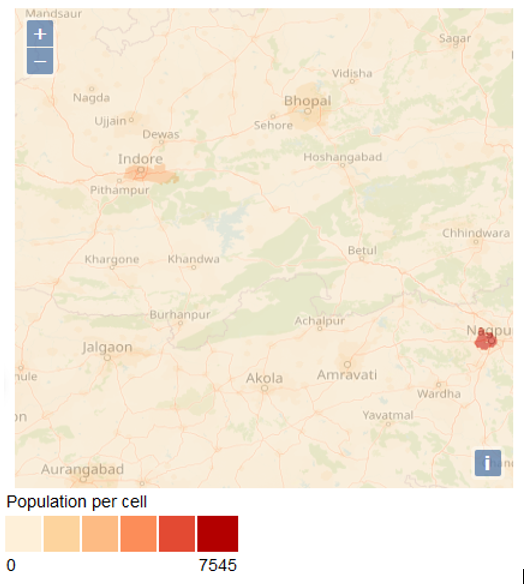
\includegraphics[width=.8\textwidth]{Pictures/MapWithWrongResolution}
 	\caption{The map looking right, but with tiles from the wrong zoom level}
 	\label{MapWithWrongResolution}
 \end{figure}


While the map appeared to look alright, it was loading tiles from the wrong zoom level. The tiles always got loaded from a zoom level 3 lower than intended. So the map in figure x is visualizing the map at zoom level 7 but loading and displaying tiles from zoom level 4.

Some experiments with loading the tiles from the correct zoom level 
Setting up Openlayers to download tile from the current view and correct zoom level chrashed the map with the error message “Insufficient Resources”. The amount of loaded tiles seems unnecessarily high and size of the tiles too small. This seems to indicate, that the tiles, which the modified version of gdal2tiles associates with zoom level 7 in fact belongs to a higher zoom level.

The reason for this bug was never discovered and the bug never got fixed. When the resolution data was gathered from the metadata file, the difference between the loaded and the actual zoom level would between different sets of tiles. This variance would depend on the which zoom levels were not being generated. So, if only the zoom levels 2-7 were generated, the difference would increase by one for each missing layer. In this case the loaded tiles would instead be wrong by 5, calculated as the default wrongness of 3 plus 2 for missing zoom layer 0 and 1. 
This bug will be defining for the rest of the code.



\section{Calculate max value in current extent}
Calculating the highest value in the current extent can be divided into two smaller tasks. Figuring out which tiles currently are being displayed and processing these tiles.

\subsection{Current displayed tiles}

The tiles, which currently is within the view, can be found using the Openlayers tileGrid method forEachTileCoord. This method can trigger a function for each tile within a given zoom level and extent. 
%https://openlayers.org/en/latest/apidoc/module-ol_tilegrid_TileGrid-TileGrid.html#forEachTileCoord
The method is going through the tiles based on their coordinates, but this can be translated to the tile urls using the getTileUrlFunction.
var tileUrlFunction = wmslayer.getSource().getTileUrlFunction()
var zoomlevelAdjustment = 3
wmslayer.getSource().getTileGrid().forEachTileCoord(loadExtent, mapZoom - zoomlevelAdjustment, function(tileCoord) {
tileName = tileUrlFunction(tileCoord, ol.proj.get('EPSG:4326'))
%Find max value
}
forEachTileCoord is triggering for each tile in the given zoom extent. This means that it on zoom level 7 it would load the tiles, that should be rendered on zoom level 7. Due to the bug mentioned section x it is not the tiles from that zoom level, which are being displayed. Instead the tiles from zoom level 2 are being displayed. This will complicate some of the next steps. 
The adjustment to the zoom level is in order to load the tiles, which should have displayed.

\subsection{Max value for each tile}
If the tiles added to the map had been from the correct zoom level calculating max value of a tile could have been done as olGeoTiff were running. olGeoTiff holds the values for the tiles in a dataarray already, so finding the maximum value could be done with a single line adding a tiles max value to the dictionary for that tile. This line is shown in code x, where urlToTiff is the name of the object, which holds the data.
        maxValueTileData[url].maxValue = Math.max(...urlToTiff[url][0])
However, since olGeoTiff holds data from an incorrect zoom layer this would not function. A possible solution would be to trigger forEachTileCoord for the same wrong zoom layer as the displayed tiles are from. This solution was not implemented since it would result in a map with could potentially so misleading information. The explanation for this has been illustrated in figure x. 

Todo: Figure with showing how large the loaded tiles are compared with how large they should be.

The tiles from the wrong zoom level are so large, that they would show data outside the view of the map. This means that the coloring could be based on the information that was outside of the current view.

The alternative solution is to run another function going through the tiles, which should have been displayed and find the highest value among these. This would result in a map where the wrong tiles were being colored based on information from the smaller correct tiles. This solution is by no means ideal. It means requesting tiles from two layers, one for displaying on the map a one for calculating the relevant max values. Loading more data than necessary will make the script slower, but since no better solution was not found this have been implemented.
The calculation of the maximum value for each tile was done in a very similar fashion to how olGeoTiff operates as illustrated in figure \ref{CalculateMaxValue}. An object holds information about all tiles, which have been processed and the max value is known. When the function is run for a tile it first checks if the tile already has been processed. If that is not the case, then it will create an object for the data, which it then will load and parse with geotiff.js. The data array with parsed data will then be run through as descripted in code x to calculate the maximum value. This maximum value will then be returned to the map. 

 
\begin{figure} [H]
	\centering
	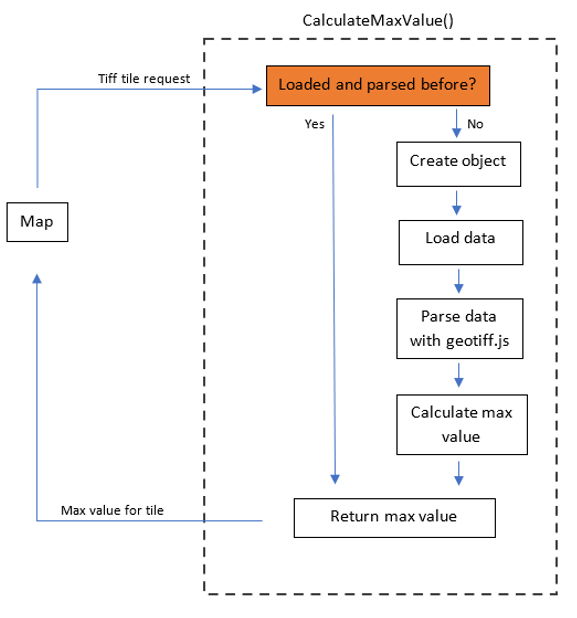
\includegraphics[width=.8\textwidth]{Pictures/CalculateMaxValue}
	\caption{Flow diagram of the calculation over max value in a tile}
	\label{CalculateMaxValue}
\end{figure}



\subsection{Highest tile value the current displayed}


To find the largest tile value among all the currently displayed tiles forEachTileCoord as mentioned earlier is used. forEachTileCoord does not have a trigger for when it has run through all the tiles. This functionality is necessary for ensuring that the produced maximum value is actually the maximum value. Without a precise end trigger the coloring applied to the map could be based on the biggest value found before the coloring script stated running instead of the absolute highest value in the current display.
Since this trigger is necessary it has been created by running forEachTileCoord another time to count the number of tiles. This part of the code can be seen in code x. 
  var tileNumber = 0;
  wmslayerMap1.getSource().getTileGrid().forEachTileCoord(loadExtent, mapZoom - zoomlevelAdjustment, function(tileCoord) {
    tileNumber++;
  })
The total number of tiles in the current extent can then be used as a trigger. 
The recoloring of the map can then be delayed until the function for calculating the maximum value have been running for the same amount of times as there are tiles on the map. In practical terms this can be accomplished by adding a counter and an if statement to the maximum-value-function. The counter would check how many times the function has run. The if statement would check if the amount of time the function had been run was equal to the number of tiles. If this is the case and the registered max value is different from the previous one the recolor function would trigger.
The calculation of the maximum value is the function presented in figure \ref{DoubleLoop}. It is running asynchronously because the array otherwise would be filled with “undefined” values instead of actual values. Running it asynchronously ensures that the script awaits the calculation of the value.  
 \begin{figure} [H]
 	\centering
 	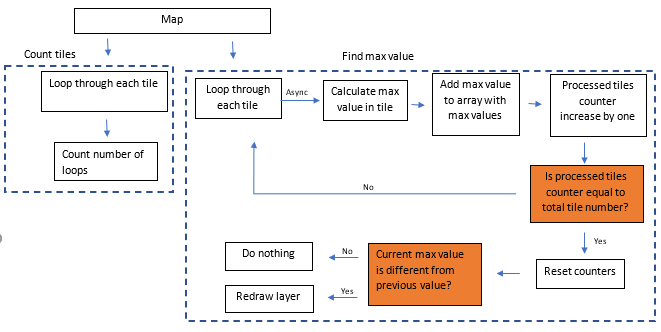
\includegraphics[width=.8\textwidth]{Pictures/DoubleLoop}
 	\caption{Finding the largest value in all currently displayed tiles}
 	\label{DoubleLoop}
 \end{figure}

\section{Recolor when the max value change}

The recoloring function was already part of olGeoTiff. However, in Bernhard Baumrocks’ thesis this recoloring was triggered manually by the user when changing the color sliders. In this project the changing of colors will trigger automatically. The function for recoloring the map have therefore been set up to trigger on the user stopping this changing the view. By not triggering before the map movement is finished a smoother user experience is ensured, since new tiles does not have to processed before the user is finished with interacting with the map. The recolor function is running through all of the code mentioned in the previous sections. 

\begin{lstlisting}[language=JavaScript, caption={The JavaScript in the project}, label= VoresJS,escapechar=|]
  map.on("moveend", function() {
    recolorMap()
  });
});
\end{lstlisting}
\section{Polish}
In addition to the rendering of the raster in the map, some features were also added to improve the user experience.


\subsection{Two maps}

\begin{figure} [H]
	\centering
	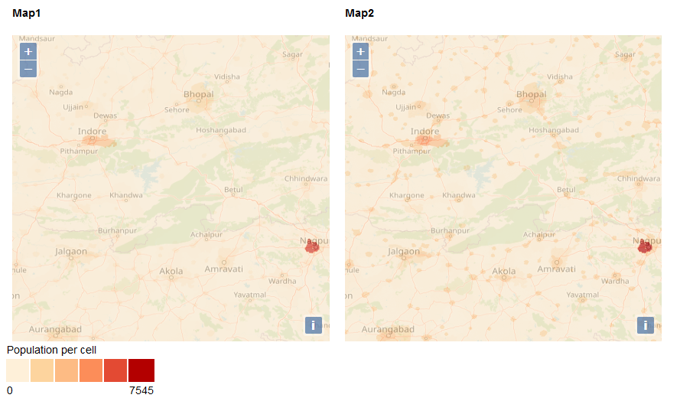
\includegraphics[width=.8\textwidth]{Pictures/DualMaps}
	\caption{A second map}
	\label{DualMaps}
\end{figure}
To be able to compare different rasters with eachother a second map was added as illustrated in figure \ref{DualMaps}. This second map is having its own raster dataset but sharing the view with the first map. This means that the two maps would always show the same area. Panning or zooming in one map would do the same action in the other map. The two maps are sharing the same legend. 
 

%Add to dualmaps how the double evaluation for multiple maps were build 

\subsection{Search function}
In order to be able to faster navigate the map a search function was created as shown in figure \ref{SearchBar}. 
 
 \begin{figure} [H]
 	\centering
 	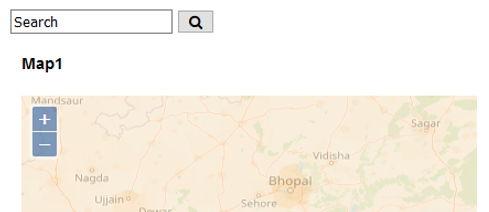
\includegraphics[width=.8\textwidth]{Pictures/SearchBar}
 	\caption{A searchbar}
 	\label{SearchBar}
 \end{figure}
 
The user can use this to change the current view of the maps to a given location. This is accomplished through the help of Nominatim. This tool can search through Openstreetmap data by location names. It then returns data about the searched location. 
https://wiki.openstreetmap.org/wiki/Nominatim

Among this data is the latitude and longitude for the central point of the place.    
%https://nominatim.openstreetmap.org/details.php?osmtype=N&osmid=245709027&class=place
This coordinate is then used as the coordinate for the center of the map.

